% Editable Beamer source. Compile with Tectonic or pdflatex (twice).
% Critic numbers: docs/results/critic_c2.md (run dir named there).
\documentclass[aspectratio=169,10pt]{beamer}
\usetheme{metropolis}
\metroset{sectionpage=none,numbering=none}
\usepackage[utf8]{inputenc}
\usepackage[T1]{fontenc}
\usepackage{booktabs,array,tabularx,amsmath,amssymb,graphicx,xcolor,tikz}
\usetikzlibrary{arrows.meta,positioning,fit,backgrounds,calc}
\setbeamercolor{background canvas}{bg=white}
\setbeamertemplate{frame footer}{RL setup optimisation -- progress}
\setbeameroption{hide notes}
\newcommand{\smallnote}[1]{{\footnotesize\color{gray}#1}}
\tikzset{box/.style={draw,rounded corners=2pt,align=center,font=\footnotesize,inner sep=4pt,fill=white},
  arr/.style={-{Stealth[length=2mm]},thick},
  grp/.style={draw=gray,dashed,rounded corners=4pt,inner sep=6pt}}
\begin{document}

% ---------------------------------------------------------------- critic 1/3
\begin{frame}{Setup critic: data and architecture}
\begin{columns}[T,onlytextwidth]
\column{.47\textwidth}
\textbf{Data} (F1\,25 and F1\,26, f1laps.com)
\begin{itemize}\setlength\itemsep{1mm}\small
\item 20{,}198 dry setups, 15 knobs mapped to Open Car Dynamics units
\item Label: \% gap to the track/session median lap
\item Driver style: 12 numbers from Time-Trial telemetry (braking 4, throttle 2, steering 3, line 3)
\item Driver, session, controller, date: training-only terms, never in $Q$
\item Folds: unseen cells, unseen drivers (person-grouped across games)
\end{itemize}
\column{.5\textwidth}
\centering
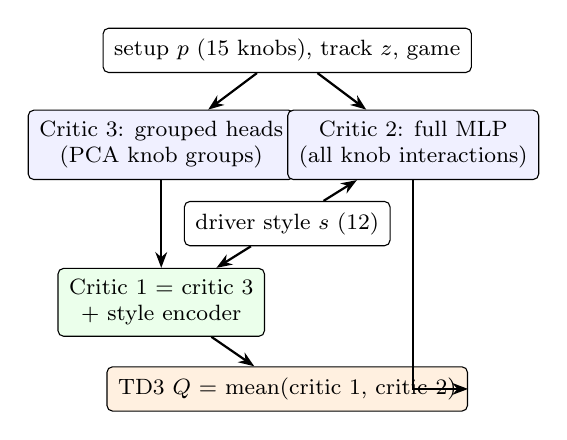
\begin{tikzpicture}
\node[box] (inp) at (1.9,0) {setup $p$ (15 knobs), track $z$, game};
\node[box,fill=blue!6] (c3) at (0.3,-1.2) {Critic 3: grouped heads\\(PCA knob groups)};
\node[box,fill=blue!6] (c2) at (3.5,-1.2) {Critic 2: full MLP\\(all knob interactions)};
\node[box] (s) at (1.9,-2.2) {driver style $s$ (12)};
\node[box,fill=green!8] (c1) at (0.3,-3.2) {Critic 1 = critic 3\\+ style encoder};
\node[box,fill=orange!12] (q) at (1.9,-4.3) {TD3 $Q$ = mean(critic 1, critic 2)};
\draw[arr] (inp) -- (c3); \draw[arr] (inp) -- (c2); \draw[arr] (c3) -- (c1);
\draw[arr] (s) -- (c1); \draw[arr] (s) -- (c2); \draw[arr] (c1) -- (q); \draw[arr] (c2) |- (q);
\end{tikzpicture}
\end{columns}
\vspace{2mm}
\smallnote{Both members of $Q$ keep the driver-style input and are smooth in $p$, so TD3 can follow $\partial Q/\partial p$.}
\end{frame}

% ---------------------------------------------------------------- critic 2/3
\begin{frame}[shrink=8]{Setup critic: ranking accuracy}
\small Pair accuracy: for two setups of the same driver, track and session, how often the critic picks the faster one (chance $=0.5$).
\vspace{2mm}

\begin{tabularx}{\textwidth}{@{}Xccc@{}}
\toprule
Model (setup part only) & Unseen cells & Unseen drivers & Barcelona\\
\midrule
Ridge baseline & 0.568 & 0.566 & --\\
Critic 3, grouped heads & 0.581 & 0.566 & 0.599\\
Critic 2 network, no style & 0.583 & 0.571 & 0.608\\
\textbf{Ensemble (delivered TD3 $Q$)} & \textbf{0.587} & \textbf{0.576} & \textbf{0.614}\\
\bottomrule
\end{tabularx}
\vspace{3mm}
\begin{itemize}\setlength\itemsep{1mm}\small
\item All pre-registered ranking bars pass (pair accuracy $\ge 0.56$, CI low $>0.52$, beats ridge, held-out setups $R^2$ gain $>0$).
\item Ensemble vs critic 3: $+0.007$ (unseen cells), $+0.010$ (unseen drivers); CIs just include 0.
\item Style path shrunk one ladder level to keep ranking safe; a gain from style is not yet detectable (MDE $\approx 0.04$).
\end{itemize}
\smallnote{3 repeats $\times$ 5 folds; 95\% person-cluster bootstrap CIs. Barcelona (unseen cells): 158 pairs, MDE $\approx 0.13$.}
\end{frame}

% ---------------------------------------------------------------- critic 3/3
\begin{frame}[shrink=3]{What limits the accuracy}
\begin{columns}[T,onlytextwidth]
\column{.52\textwidth}
\centering
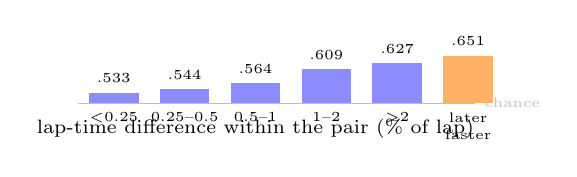
\begin{tikzpicture}[x=9mm,y=40mm]
\draw[gray!50] (0,.5) -- (5.6,.5) node[right,font=\tiny]{chance};
\foreach \i/\v/\lab in {0/.533/{$<$0.25},1/.544/{0.25--0.5},2/.564/{0.5--1},3/.609/{1--2},4/.627/{$>$2}}{
  \fill[blue!45] (\i+.15,.5) rectangle (\i+.85,\v);
  \node[above,font=\tiny] at (\i+.5,\v) {\v};
  \node[below,font=\tiny] at (\i+.5,.5) {\lab};}
\fill[orange!60] (5.15,.5) rectangle (5.85,.651); \node[above,font=\tiny] at (5.5,.651) {.651};
\node[below,font=\tiny,align=center] at (5.5,.5) {later\\faster};
\node[font=\scriptsize] at (2.5,.42) {lap-time difference within the pair (\% of lap)};
\end{tikzpicture}
\column{.45\textwidth}
\small
\begin{itemize}\setlength\itemsep{1.5mm}
\item Clear differences ($>1\%$) and same-day pairs: \textbf{0.61--0.63}.
\item Tiny differences ($<0.25\%$): near chance --- lap noise.
\item ``The later setup is faster'' alone: 0.651. Most within-driver change is the driver improving, not the setup.
\item Date is kept out of $Q$: TD3 cannot change it.
\item Tried without gain: pairwise ranking loss, wider nets, seed ensembles (plateau $\approx 0.58$).
\end{itemize}
\end{columns}
\vspace{2mm}
\smallnote{Chart: ensemble, first run (20{,}190 setups). Cleaner labels need several laps per setup on the same day: OCD and Assetto Corsa runs provide them.}
\end{frame}

% ---------------------------------------------------------------- TD3 1/2
\begin{frame}{TD3 setup agent: proposed architecture}
\centering
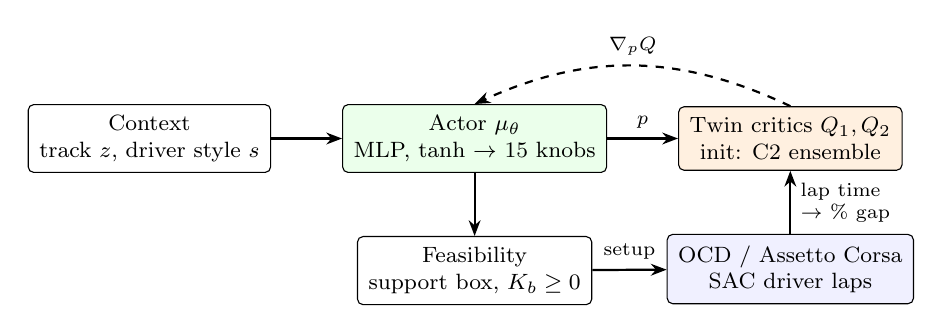
\begin{tikzpicture}[node distance=5mm and 9mm]
\node[box] (ctx) {Context\\track $z$, driver style $s$};
\node[box,right=of ctx,fill=green!8] (actor) {Actor $\mu_\theta$\\MLP, $\tanh$ $\to$ 15 knobs};
\node[box,right=of actor,fill=orange!12] (q) {Twin critics $Q_1,Q_2$\\init: C2 ensemble};
\node[box,below=8mm of actor] (feas) {Feasibility\\support box, $K_b \ge 0$};
\node[box,below=8mm of q,fill=blue!6] (sim) {OCD / Assetto Corsa\\SAC driver laps};
\draw[arr] (ctx) -- (actor); \draw[arr] (actor) -- node[above,font=\scriptsize]{$p$} (q);
\draw[arr] (actor) -- (feas); \draw[arr] (feas) -- node[above,font=\scriptsize]{setup} (sim);
\draw[arr] (sim) -- node[right,font=\scriptsize,align=left]{lap time\\$\to$ \% gap} (q);
\draw[arr,dashed] (q.north) to[bend right=25] node[above,font=\scriptsize]{$\nabla_p Q$} (actor.north);
\end{tikzpicture}
\vspace{3mm}
\begin{itemize}\setlength\itemsep{1mm}\small
\item One-step problem (bandit, $\gamma=0$): state = track + driver style, action = setup, reward $= -$lap-time gap.
\item TD3 parts kept: twin critics with $\min(Q_1,Q_2)$, target policy smoothing, delayed actor updates.
\item Actor penalised outside the data's support box; style clipped to the training range.
\end{itemize}
\end{frame}

% ---------------------------------------------------------------- TD3 2/2
\begin{frame}{TD3 setup agent: plan}
\begin{tabularx}{\textwidth}{@{}l X@{}}
\toprule
Step & Content\\
\midrule
1. Offline actor & Train $\mu_\theta$ against the frozen C2 ensemble on Barcelona and the other tracks; check proposed setups stay in support.\\
2. Sanity check & Compare the actor's setups with the community meta setups and with critic ranking of known good setups.\\
3. Online loop (OCD) & Each proposed setup is driven by the SAC driver; the lap is added to the data and the critics are fine-tuned (Barcelona head).\\
4. Assetto Corsa & Same loop through the Lenovo collector; few laps, so screen candidates with $Q$ first.\\
5. Evaluation & Lap time vs default and meta setups; per driver style (attacker, smooth, neutral).\\
\bottomrule
\end{tabularx}
\vspace{3mm}
\smallnote{Open: measured game$\to$OCD knob constants, recorded Barcelona track edges, target session (solo hot lap).}
\end{frame}

% ---------------------------------------------------------------- TCP
\begin{frame}{Assetto Corsa training: Lenovo $\leftrightarrow$ Mac}
\centering
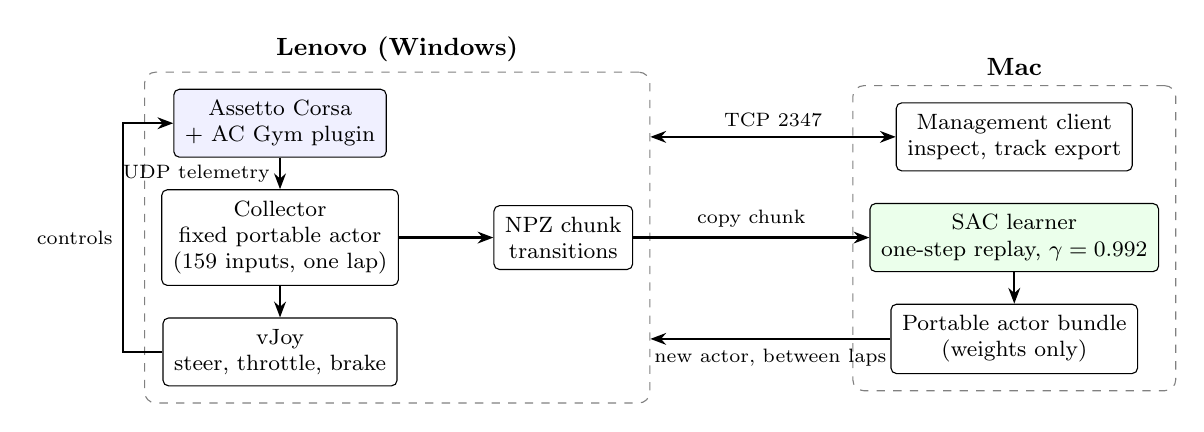
\begin{tikzpicture}[node distance=4mm and 6mm]
\node[box,fill=blue!6] (ac) {Assetto Corsa\\+ AC Gym plugin};
\node[box,below=of ac] (col) {Collector\\fixed portable actor\\(159 inputs, one lap)};
\node[box,below=of col] (vj) {vJoy\\steer, throttle, brake};
\node[box,right=12mm of col] (npz) {NPZ chunk\\transitions};
\begin{scope}[on background layer]
\node[grp,fit=(ac)(col)(vj)(npz),label={[font=\small\bfseries]above:Lenovo (Windows)}] (len) {};
\end{scope}
\node[box,right=30mm of npz,fill=green!8] (sac) {SAC learner\\one-step replay, $\gamma=0.992$};
\node[box,above=of sac] (mgmt) {Management client\\inspect, track export};
\node[box,below=of sac] (bund) {Portable actor bundle\\(weights only)};
\begin{scope}[on background layer]
\node[grp,fit=(sac)(mgmt)(bund),label={[font=\small\bfseries]above:Mac}] (mac) {};
\end{scope}
\draw[arr] (ac) -- node[left,font=\scriptsize]{UDP telemetry} (col);
\draw[arr] (col) -- (vj); \draw[arr] (vj.west) -- ++(-.5,0) |- node[pos=.25,left,font=\scriptsize]{controls} (ac.west);
\draw[arr] (col) -- (npz);
\draw[arr] (npz) -- node[above,font=\scriptsize]{copy chunk} (sac);
\draw[arr,{Stealth[length=2mm]}-{Stealth[length=2mm]}] (mgmt.west) -- node[above,font=\scriptsize]{TCP 2347} (mgmt.west -| len.east);
\draw[arr] (sac) -- (bund);
\draw[arr] (bund.west) -- node[below,font=\scriptsize]{new actor, between laps} (bund.west -| len.east);
\end{tikzpicture}
\end{frame}

\end{document}
